\documentclass{beamer}
%\setbeamersize{text margin left=30mm,text margin right=30mm} 
%\setbeamertemplate{frametitle}{\vspace{2cm} \\ \insertframetitle }
%\setbeamertemplate{footline}{\vspace{0.5cm}}
%\addtolength{\headsep}{-16cm}



% The Beamer class comes with a number of default slide themes
% which change the colors and layouts of slides. Below this is a list
% of all the themes, uncomment each in turn to see what they look like.
\mode<presentation> {
\usetheme{Marburg}
\usecolortheme{orchid}
}
%\addtobeamertemplate{beamercolorbox}{}{\vspace{-20em}}

%\usepackage{bbm}


\usepackage{float}
%\usepackage[cmbold]{mathtime}
%\usepackage{mt11p}
\usepackage{placeins}
\usepackage{amsmath}
\usepackage{color}
\usepackage{amssymb}
\usepackage{mathtools}
\usepackage{subfigure}
\usepackage{multirow}
\usepackage{epsfig}
\usepackage{listings}
\usepackage{enumitem}
\usepackage{rotating,tabularx}
%\usepackage[graphicx]{realboxes}
\usepackage{graphicx}
\usepackage{graphics}
\usepackage{epstopdf}
\usepackage{longtable}
%\usepackage{smartdiagram}
%\usepackage[pdftex]{hyperref}
%\usepackage{breakurl}
%\usepackage{epigraph}
%\usepackage{xspace}
\usepackage{amsfonts}
\usepackage{eurosym}
%\usepackage{ulem}
\usepackage{footmisc}
%\usepackage{comment}
\usepackage{setspace}
\usepackage{geometry}
\usepackage{caption}
%\usepackage{pdflscape}
\usepackage{array}
\usepackage[round]{natbib}
\usepackage{booktabs}
\usepackage{dcolumn}
\usepackage{mathrsfs}
%\usepackage[justification=centering]{caption}
%\captionsetup[table]{format=plain,labelformat=simple,labelsep=period,singlelinecheck=true}%

%\bibliographystyle{unsrtnat}
%\bibliographystyle{aea}
\usepackage{enumitem}
\usepackage{tikz}
\def\checkmark{\tikz\fill[scale=0.4](0,.35) -- (.25,0) -- (1,.7) -- (.25,.15) -- cycle;}
%\usepackage{tikz}
%\usetikzlibrary{snakes}
%\usetikzlibrary{patterns}

%\draftSpacing{1.5}

\usepackage{xcolor}
\hypersetup{
colorlinks,
linkcolor={blue!50!black},
citecolor={blue!50!black},
urlcolor={blue!50!black}}

%\renewcommand{\familydefault}{\sfdefault}
%\usepackage{helvet}
%\setlength{\parindent}{0.4cm}
%\setlength{\parindent}{2em}
%\setlength{\parskip}{1em}

%\normalem

%\doublespacing
%\onehalfspacing
%\singlespacing
%\linespread{1.5}

%\newtheorem{theorem}{Theorem}
%\newtheorem{corollary}[theorem]{Corollary}
\newtheorem{proposition}{Proposition}
%\newtheorem{definition}{Definition}
\newtheorem{axiom}{Axiom}
\newcommand{\ra}[1]{\renewcommand{\arraystretch}{#1}}

\newcommand{\E}{\mathrm{E}}
\newcommand{\Var}{\mathrm{Var}}
\newcommand{\Corr}{\mathrm{Corr}}
\newcommand{\Cov}{\mathrm{Cov}}

\newcolumntype{d}[1]{D{.}{.}{#1}} % "decimal" column type
\renewcommand{\ast}{{}^{\textstyle *}} % for raised "asterisks"

\newtheorem{hyp}{Hypothesis}
\newtheorem{subhyp}{Hypothesis}[hyp]
\renewcommand{\thesubhyp}{\thehyp\alph{subhyp}}

\newcommand{\red}[1]{{\color{red} #1}}
\newcommand{\blue}[1]{{\color{blue} #1}}

%\newcommand*{\qed}{\hfill\ensuremath{\blacksquare}}%

\newcolumntype{L}[1]{>{\raggedright\let\newline\\arraybackslash\hspace{0pt}}m{#1}}
\newcolumntype{C}[1]{>{\centering\let\newline\\arraybackslash\hspace{0pt}}m{#1}}
\newcolumntype{R}[1]{>{\raggedleft\let\newline\\arraybackslash\hspace{0pt}}m{#1}}

%\geometry{left=1.5in,right=1.5in,top=1.5in,bottom=1.5in}
%\geometry{left=1in,right=1in,top=1in,bottom=1in}

\epstopdfsetup{outdir=./}

\newcommand{\elabel}[1]{\label{eq:#1}}
\newcommand{\eref}[1]{Eq.~(\ref{eq:#1})}
\newcommand{\ceref}[2]{(\ref{eq:#1}#2)}
\newcommand{\Eref}[1]{Equation~(\ref{eq:#1})}
\newcommand{\erefs}[2]{Eqs.~(\ref{eq:#1}--\ref{eq:#2})}

\newcommand{\Sref}[1]{Section~\ref{sec:#1}}
\newcommand{\sref}[1]{Sec.~\ref{sec:#1}}

\newcommand{\Pref}[1]{Proposition~\ref{prop:#1}}
\newcommand{\pref}[1]{Prop.~\ref{prop:#1}}
\newcommand{\preflong}[1]{proposition~\ref{prop:#1}}

\newcommand{\Aref}[1]{Axiom~\ref{ax:#1}}

\newcommand{\clabel}[1]{\label{coro:#1}}
\newcommand{\Cref}[1]{Corollary~\ref{coro:#1}}
\newcommand{\cref}[1]{Cor.~\ref{coro:#1}}
\newcommand{\creflong}[1]{corollary~\ref{coro:#1}}

\newcommand{\etal}{{\it et~al.}\xspace}
\newcommand{\ie}{{\it i.e.}\ }
\newcommand{\eg}{{\it e.g.}\ }
\newcommand{\etc}{{\it etc.}\ }
\newcommand{\cf}{{\it c.f.}\ }
\newcommand{\ave}[1]{\left\langle#1 \right\rangle}
\newcommand{\person}[1]{{\it \sc #1}}

\newcommand{\AAA}[1]{\red{{\it AA: #1 AA}}}
\newcommand{\YB}[1]{\blue{{\it YB: #1 YB}}}

\newcommand{\flabel}[1]{\label{fig:#1}}
\newcommand{\fref}[1]{Fig.~\ref{fig:#1}}
\newcommand{\Fref}[1]{Figure~\ref{fig:#1}}

\newcommand{\tlabel}[1]{\label{tab:#1}}
\newcommand{\tref}[1]{Tab.~\ref{tab:#1}}
\newcommand{\Tref}[1]{Table~\ref{tab:#1}}

\newcommand{\be}{\begin{equation}}
\newcommand{\ee}{\end{equation}}
\newcommand{\bea}{\begin{eqnarray}}
\newcommand{\eea}{\end{eqnarray}}

\newcommand{\bi}{\begin{itemize}}
\newcommand{\ei}{\end{itemize}}

\newcommand{\Dt}{\Delta t}
\newcommand{\Dx}{\Delta x}
\newcommand{\Epsilon}{\mathcal{E}}
\newcommand{\etau}{\tau^\text{eqm}}
\newcommand{\wtau}{\widetilde{\tau}}
\newcommand{\xN}{\ave{x}_N}
\newcommand{\Sdata}{S^{\text{data}}}
\newcommand{\Smodel}{S^{\text{model}}}

\newcommand{\del}{D}
\newcommand{\hor}{H}

\setlength{\parindent}{0.0cm}
\setlength{\parskip}{0.4em}

\numberwithin{equation}{section}
\DeclareMathOperator\erf{erf}
%\let\endtitlepage\relax

%\mode<presentation> {

% The Beamer class comes with a number of default slide themes
% which change the colors and layouts of slides. Below this is a list
% of all the themes, uncomment each in turn to see what they look like.

% As well as themes, the Beamer class has a number of color themes
% for any slide theme. Uncomment each of these in turn to see how it
% changes the colors of your current slide theme.

%\usecolortheme{albatross}
%\usecolortheme{beaver}
%\usecolortheme{beetle}
%\usecolortheme{crane}
%\usecolortheme{dolphin}
%\usecolortheme{dove}
%\usecolortheme{fly}
%\usecolortheme{lily}
%\usecolortheme{orchid}
%\usecolortheme{rose}
%\usecolortheme{seagull}
%\usecolortheme{seahorse}
%\usecolortheme{whale}
%\usecolortheme{wolverine}

%\setbeamertemplate{footline} % To remove the footer line in all slides uncomment this line
%\setbeamertemplate{footline}[page number] % To replace the footer line in all slides with a simple slide count uncomment this line


%----------------------------------------------------------------------------------------
%   TITLE PAGE
%----------------------------------------------------------------------------------------

\title[Direction of innovation]{Direction of Innovation} % The short title appears at the bottom of every slide, the full title is only on the title page

\author{Diomides Mavroyiannis} % Your name
\institute[Paris Dauphine] % Your institution as it will appear on the bottom of every slide, may be shorthand to save space
{
PSL/Paris Dauphine \\ % Your institution for the title page
\medskip% Your email address
}
\date{\today}

\begin{document}

\begin{frame}
\titlepage % Print the title page as the first slide
\end{frame}


\section{Introduction}
%------------------------------------------------
\subsection{Motivation}
\begin{frame}{Motivation}
\begin{itemize}
    \item \textbf{Definition:} A buyout will be used to refer to the purchase of technological assets
    \item Buyouts are prevalent, the basic effect of buyouts is that they decrease the price elasticity of the market.  
    \item From an economic theory point of view, buyouts are a double edged sword.  
    \item \textbf{Positive:} Increase potential payoff for entrepreneurs, more projects undertaken, more innovation
    \item \textbf{Negative:} Increases monopoly power
    \item Sometimes buyouts can occur without these side effects, value buyers. 
\end{itemize}
\end{frame}

\subsection{Literature review}

%%%%%%%%%%%%%%%%%%%%%%%%%%%%%%%%%%%%%%%%%%%%%%%%%%%%%%%%%%%%%

\begin{frame}{Literature review}
\begin{itemize}
    \item Empirically firms which are less innovative are more likely to engage in buyouts. Higgins and Rodriguez (2006) and Zhao (2009)
    \item Coase theorem works here because substitutability can be framed in terms of externalities.See Kuechle $\&$ Rios  (2012)
    \item Large firms avoid engaging in competition effects, Aghion (2005)
    \item Cabal (2003) has an R$\&$D race where two firms choose R$\&$D technologies. 
\end{itemize}
\end{frame}

\subsection{Assumptions}

\begin{frame}{Firms and cost structure}
\begin{itemize}
    \item There are two firms, an entrant($c_e$) and incumbent($c_i$) competition
    \item Two potential future costs: intermediate $c_1$  and advanced $c_2$
    \item Firms only use the best technology available to them. Incumbent technology is only inferior to the advanced tech. $\pi_{i}(c_{i},c_{e2})>\pi_{i}(c_{i1},c_{e2})$
    \item The entrant technology is inferior to both other technologies. $\pi_{e}(c_{i},c_{e1})>\pi_{i}(c_{i},c_{e})$
    \item \textbf{Timing:} \\
    Negotiation $\rightarrow$  Incumbent chooses  $\rightarrow$ competition(a priori)
    Entrant chooses $\rightarrow$ negotiation $\rightarrow$ competition(a posteriori)
\end{itemize}
\end{frame}

\begin{frame}{Sub-additive competitive profits}
\begin{itemize}
	\item Monopoly assumption
	\item Pesky Entrant
\end{itemize}
\begin{equation*}
\pi_{i}(c_{i2},c_{e}) \geq  \pi_{i}(c_{i},c_{e2}) + \pi_{e}(c_{i},c_{e2})
\end{equation*}
\begin{equation*}
\pi_{i}(c_{i},c_{e}) \geq  \pi_{i}(c_{i},c_{e1}) + \pi_{e}(c_{i},c_{e1})
\end{equation*}
\end{frame}

\subsubsection{Technology}
\subsubsection{Sequential}
\begin{frame}{Sequential}
\begin{itemize}
    \item \textbf{Entrant payoff}: $\pi_e(c_i,c_{i1}) (t_2-t_1) +\pi_e(c_i,c_{e2})(T+1-t_2)$
    \item \textbf{Incumbent payoff}: $\pi_i(c_i,c_{e})t_1+\pi_i(c_i,c_{i1}) (t_2-t_1)+\pi_i(c_i,c_{e2})(T+1-t_2)$
    \item \textbf{Monopoly payoff}:  
    \item $\pi_i(c_i,c_{e}) t_2+\pi_i(c_{i2},c_e)(T+1-t_2)$
\end{itemize}
\end{frame}

\subsubsection{Technology}
\subsubsection{Sequential}
\begin{frame}{Sequential}
\begin{align*}
WTP=\Pi_{s}^m-\Pi_{is} = (\pi_i(c_i,c_{e})-\pi_i(c_i,c_{i1}))(t_2-t_1)+(\pi_i(c_{i2},c_e)-\pi_i(c_{i},c_{e2}))(T+1-t_2) \\
S_s= (\pi_i(c_i,c_{e})-\pi_i(c_i,c_{i1})-\pi_e(c_i,c_{i1}))(t_2-t_1)+(\pi_i(c_{i2},c_e)-\pi_i(c_{i},c_{e2})-\pi_e(c_{i},c_{e2}))(T+1-t_2) \\
B_{es}(\omega)=\Pi_{es}+ \omega S_s  \\
\end{align*}
\end{frame}

\subsubsection{Technology}
\begin{frame}{Model:Technology}
\begin{itemize}
    \item The sequential technology takes two periods to innovate. In the first period the entrants cost is $c_{1}$ and in the second it is $c_{2}$
    \item In the radical technology, with probability q, the cost will be $c_{2}$ in the first period.
    \item If the technology fails then with probability q it will succeed in the second period. 
\end{itemize}
\end{frame}



\subsection{A priori buyout}

\begin{frame}{A priori}
\begin{block}{A priori cutoff}
If the buyouts are priori, the decision criteria for the radical innovation to be chosen by the incumbent is: 
\begin{equation*}
\frac{3-\sqrt{5}}{2}<q^{p}
\end{equation*}
\end{block}

\begin{proof}
We need only set: 
\begin{align*}
\Pi_{IR}^m >\Pi_{IS}^m \\
\pi_{i}^m (1-q) (2-q)+\pi_{i2}^m q (3-q)>\pi_{i}^m +  \pi_{i2}^m 
\end{align*}
\end{proof}
\end{frame}


\section{Bertrand}
\subsubsection{Sequential}
\begin{frame}{Bertrand: Sequential}
\begin{itemize}
    \item The market profits of the incumbent in the sequential technology case is:
    \begin{equation*}
        \overline{\Pi}_{IS} = \pi_{i1}=(1-c_{i1})(c_{i1}-c_i) 
    \end{equation*}
    \item The market payoffs of the entrant 
    \begin{equation*}
        \overline{\Pi}_{ES} =  
 \pi_{e2}=(1-c_{i})(c_i-c_{e2}) 
    \end{equation*}
    \item The monopoly profit of the incumbent with a buyout is
    \begin{equation*}
        \Pi_{IS} = \pi_{i} +  \pi_{i2} 
    \end{equation*}
    \item Therefore the bargaining payoff if there is a buyout of the entrant is: 
    \begin{equation*}
       B_{ES}(\omega)=  \pi_{e2}(1-\omega)+ \omega (\pi_{i} +  \pi_{i2} - \pi_{i1} )
    \end{equation*}
\end{itemize}
\end{frame}

\begin{frame}{Model: Sequential 2}
\begin{itemize}
    \item We can also compute the difference between the entrant buyout profits to the non-buyout profits as
    \begin{equation*}
        B_{ES}(\omega) - \overline{\Pi}_{ES} = 
\omega (\pi_{i} +  \pi_{i2} - \pi_{i1}-\pi_{e2} )
    \end{equation*}
    \item This is the incentive effect of buyouts
    \item Note the effect of barganing power. 
\end{itemize}
\end{frame}

\subsubsection{Radical}

\begin{frame}{Model: Radical}
\begin{itemize}
    \item The market profits of the incumbent in the radical  technology case is:
    \begin{equation*}
       \overline{\Pi}_{IR} = (1-q)(2-q) \pi_{i}
    \end{equation*}
    \item The market payoffs of the entrant 
    \begin{equation*}
\overline{\Pi}_{ER} =
q 2 \pi_{e2}+(1-q)q\pi_{e2}=q\pi_{e2}(3-q)
    \end{equation*}
    \item The market profits of the incumbent with a buyout is
    \begin{equation*}
       \Pi_{IR} = \pi_{i} (1-q) (2-q)+\pi_{i2} q (3-q)
    \end{equation*}
    \item Therefore the bargaining payoff if there is a buyout of the entrant is: 
    \begin{equation*}
       B_{ER}(\omega)=  (3-q)q(\pi_{e2}+\omega  (\pi_{i2} - \pi_{e2}))
    \end{equation*}
\end{itemize}
\end{frame}

\begin{frame}{Model: Radical 2}
\begin{itemize}
    \item Incentive effect of the buyout is therefore:
    \begin{equation*}
B_{ER}-\overline{\Pi}_{ER} 
=\omega (3-q)q 
\left(
\pi_{i2} 
-\pi_{e2}
\right) 
    \end{equation*}
\item Notice that once again this heavily depends on bargaining power*
\end{itemize}
\end{frame}

\subsubsection{Results}

\begin{frame}{Model: Results}
\begin{block}{Proposition 1}
The entrant will choose the radical innovation over the incremental innovation if there are no buyout iff: 
\begin{equation*}
\pi_{e2}(q(3-q)-1)+k_S-k_R > 0
\end{equation*}
\end{block}
This is found simply by setting:
\begin{equation*}
\overline{\Pi}_{ER}-k_R > \overline{\Pi}_{ES}-k_S 
\end{equation*}
\end{frame}


\begin{frame}{Corollary 1}
\begin{block}{Cutoff probability}
If costs are identical then the required q for the radical innovation to prefered is given by: 
\begin{equation*}
q > \frac{3-\sqrt{5}}{2}=q^{b}
\end{equation*}
\end{block}
\end{frame}

\begin{frame}{Results 2}
\begin{block}{Proposition 2}
If costs are identical then a buyout will neccesarily require a higher $q^{b*}$ than $q^b$ to incite the entrant to pursue the radical innovation. 
\end{block}
This follows by setting 
\begin{align*}
B_{ER}(\omega)-k_R>B_{ES}(\omega)-k_S \\
\rightarrow (1-\omega) \pi_{e2}(q(3-q)-1)
+ \omega \pi_{i2} (q(3-q)-1) \\  -\omega(\pi_i- \pi_{i1})
> 0
\end{align*}
Note that the third term is negative, $-\omega(\pi_i- \pi_{i1})$, which implies higher $q$
\end{frame}

\subsubsection{Example}

\begin{frame}{Example}
\begin{itemize}
    \item Let $\pi_{e2}=40$, $\pi_{i2}=100$, $\pi_{e1}=20$ $\pi_{i}=80$. $\omega = .5, q=0.5$ \\
    \item \textbf{No buyouts Sequential:} Entrant earns $40$. \textbf{Radical} entrant earns $.5(40+40)+(.5)^2(40)=50$. \newline Radical$>$Sequential 
    \item \textbf{Buyouts, Sequential bargaining surplus:}  $NS_S = 100+80-20-40=120$. Therefore the payoff of the entrant is $40+\frac{1}{2}(120)=100$. \newline \textbf{Radical innovation surplus:} $ .5(200)+(.5)^2 180+(.5)^2 160-(.5)^2 80-(.5)^2-50=75$. Therefore the payoff after bargaining is $50+\frac{1}{2}(75)=87.5$ 
    \newline
    Sequential $>$ Radical
\end{itemize}
\end{frame}


\section{Cournot}

\subsubsection{Sequential}
\begin{frame}{Cournot: Sequential}
\begin{itemize}
    \item The market profits of the incumbent in the sequential technology case is:
    \begin{equation*}
        \overline{\Pi}_{ES} =
        \left(\frac{1-2 c_{i1}+c_{i}}{3}  \right)^2
        +
        \left(\frac{1-2 c_{i2}+c_{i}}{3}  \right)^2
    \end{equation*}
    \item The market payoffs of the entrant 
    \begin{equation*}
        \overline{\Pi}_{IS} =  
\left(\frac{1+ c_{i1}-2c_{i}}{3}  \right)^2
+ \left(\frac{1+ c_{i2}-2c_{i}}{3}  \right)^2
    \end{equation*}
    \item The monopoly profit is unchanged relative to Bertrand
\end{itemize}
\end{frame}

\begin{frame}{Cournot: Sequential 2}
\begin{itemize}
\item The Nash surplus is given by:
\begin{equation*}
NS_{S}^{c} = \pi^m+\pi^m_{2}- \pi_{i1}^{c}-\pi_{i2}^{c}-\pi_{e1}^{c}-\pi_{e2}^{c}
\end{equation*}

\item The Bargaining payoff of the entrant is: 
\begin{equation*}
B_{ES}^{c} = \Pi_{ES}^{c} + \omega NS_{S}^{c} 
\end{equation*}
    
\item The barganing payoff of the incumbent is: \begin{equation*}
B_{IS}^{c} = \Pi_{IS}^{c}+ (1-\omega) NS_{S}^{c}
\end{equation*}
\end{itemize}
\end{frame}

\subsubsection{Radical}

\begin{frame}{Model: Radical}
\begin{itemize}
    \item The market profits of the incumbent in the radical  technology case is:
    \begin{equation*}
       \overline{\Pi}_{IR} = (1-q) (2-q)\pi^{m}  + q \pi_{i1}^{c}(3-q)
    \end{equation*}
    \item The market payoffs of the entrant 
    \begin{equation*}
\overline{\Pi}_{ER} =
q \pi_{e2}^{c} (3-q)
    \end{equation*}
    \item The monopoly profits are given by:
\begin{equation*}
\Pi_{R}^{m} = \pi^{m} (1-q) (2-q)+\pi_{2}^{m} q (3-q)
\end{equation*}
\end{itemize}
\end{frame}

\begin{frame}{Cournot: Radical 2}
\begin{itemize}
\item The Nash surplus is given by:
\begin{align*}
NS_{R}^{c} = \pi^{m} (1-q) (2-q)+\pi_{2}^{m} q (3-q)- \Pi_{IR}^{c} - \Pi_{ER}^{c} \\
= q(3-q) (\pi_{2}^{m}-\pi_{e2}^{c}-\pi_{i1}^{c})
\end{align*}



\item The Bargaining payoff of the entrant is: 
\begin{equation*}
B_{ER}^{c} = \Pi_{ER}^{c} + \omega NS_{R}^{c} 
\end{equation*}
    
\item The barganing payoff of the incumbent is: \begin{equation*}
B_{IR}^{c} = \Pi_{IR}^{c} + (1-\omega) NS_{R}^{c}
\end{equation*}
\end{itemize}
\end{frame}


\subsection{Results}
\begin{frame}{Cournot no buyout cutoff}
\begin{block}{Cournot Cutoff preferences}
The cutoff point for the entrant to prefer th radical innovation without buyouts is given by: 
\begin{equation*}
\frac{3}{2}-\frac{ \sqrt{5 \pi_{e2}^{c}-4 \pi_{e1}^{c}}}{2 \sqrt{\pi_{e2}^{c}}}=q^{c}
\end{equation*}
\end{block}
Proof:
\begin{align*}
\Pi_{ER}^{c}>\Pi_{ES}^{c} \\
q \pi_{e2}^{c} (3-q) > \pi_{e1}^{c}+\pi_{e2}^{c} \\
q> 
\frac{3 \pi_{e2}^{c}-\sqrt{\pi_{e2}^{c}} \sqrt{5 \pi_{e2}^{c}-4 \pi_{e1}^{c}}}{2 \pi_{e2}^{c}} 
\end{align*}
\end{frame}

\begin{frame}{With buyout cutoff point}
\begin{block}{Cutoff with buyouts}
With buyouts, the cutoff efficiency of the radical innovation for it to be pursued is lower in Cournot competition than in Bertrand
\end{block}
\end{frame}

\subsection{Bertrand vs Cournot without buyout}
\begin{frame}{Bertrand vs Cournot}
\begin{block}{Cournot radical preferences entail Bertrand}
Without buyouts, if the radical innovation is preferred in Cournot competition, it is also preferred in Bertrand. 
\end{block}
We note that $q^c$ cutoff is strictly increasing in $\pi_{e1}^{c}$ and that if $\pi_{e1}^{c}=0$ we have the Bertrand payoff.
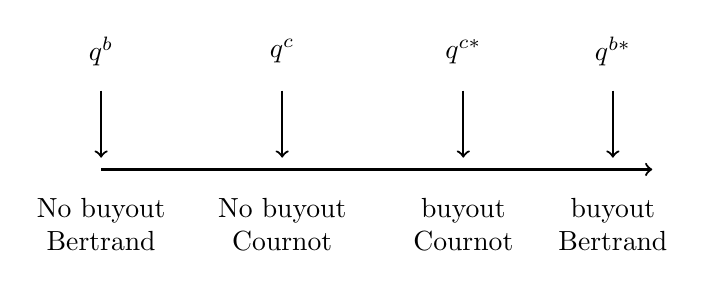
\begin{tikzpicture}[scale=1]
\node[align=center] at (0,1.5) {$q^b$};
\draw [thick,->] (0,1) -- (0,0.15);
\node[align=center] at (0,-.7) {No buyout \\ Bertrand};
%%%%%%%%%%%%%%%%
\node[align=center] at (2.3,1.5) {$q^c$};
\draw [thick,->] (2.3,1) -- (2.3,0.15);
\node[align=center] at (2.3,-.7) 
{No buyout \\ Cournot };
%%%%%%%%%%%%%%%%
%%%%%%%%%%%%%%%%
\node[align=center] at (4.6,1.5) {$q^{c*}$};
\node[align=center] at (4.6,-.7) { buyout \\ Cournot  };
\draw [thick,->] (4.6,1) -- (4.6,0.15);
%%%%%%%%%%%%%%%%
\node[align=center] at (6.5,1.5) {$q^{b*}$};
\node[align=center] at (6.5,-.7) {buyout \\ Bertrand};
\draw [thick,->] (6.5,1) -- (6.5,0.15);
%%%%%%%%%%%%%%%%
%%%%%%%%%%%%%%%%
%%%%%%%%%%%%%%%%
\draw [thick,->] (0,0) -- (7,0);
\end{tikzpicture}
\end{frame}

\section{Welfare}

\begin{frame}{Main welfare result}
\begin{block}{Welfare proposition}
The cutoff point for welfare to be maximized by radical innovation with buyouts, $q^{w*}$ is the same as the a priori cutoff point,$q^{*}$ and the posterior no buyout cutoff point, $q^{b}$
\end{block}
This follows by setting: 
\begin{equation*}
W_R> W_S \rightarrow  w_{m2}(3q-q^2-1)-w_{mI}(3q-q^2-1)>0
\end{equation*}
%welfare is only aligned if there is no bargaining power
\end{frame}


\subsection{Policy implications}


\AtBeginSection[]
{
\begin{frame}{Table of Contents}
\tableofcontents[currentsection]
\end{frame}
}


\begin{frame}{Conclusive comments }
\begin{itemize}
    \item Allowing buyouts has distortion effects on the market if the entrant has bargaining power
    \item Therefore any cost benefit analysis that evaluates the effects of buyouts should include the costs and benefits of industry diversification
    \item Intellectual property may cause industry convergence
    \item Convergence effect vs a divergence effect
\end{itemize}
\end{frame}

\begin{frame}
\bibliographystyle{aea}
\small{
\bibliography{../LML_bibliography/bibliography}}
\end{frame}


\end{document}
